\begin{figure}[ht]
	\centering
	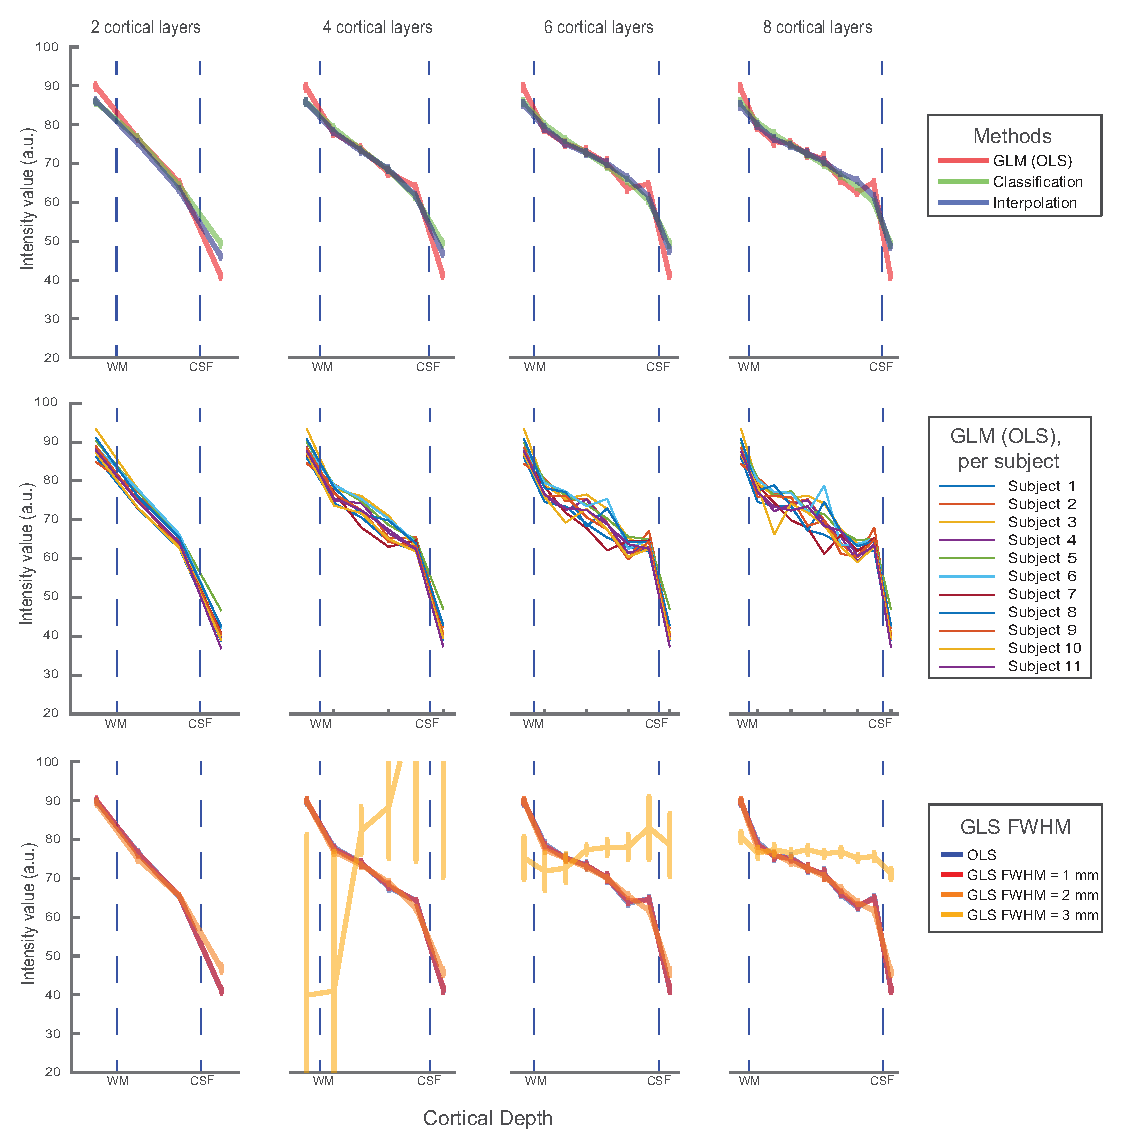
\includegraphics[width=0.9\textwidth, clip=true]{./Chapters/03_GLM/./Images/ProfileComparisons}
	\caption{The obtained profiles for a small piece of the primary visual cortex, based on 11 subjects, for a varying number of layers (columns). In the first row, the three different methods are compared. The second row shows the individual profiles for the GLM method, showing that the solution becomes unstable when higher numbers of layers are used. In the bottom row, different FWHMs are tested in a generalised least squares solution.}
	\label{fig:profileaverage}
\end{figure}